\section{Collections in COMPSs}
\label{sec:col}
As we have seen in previous sections and examples, a COMPSs parameter is basically a regular user-code object, as a \verb|numpy.ndarray|, with additional metadata to help the COMPSs Runtime to compute any dependency between tasks induced by this particular object, keep track of its locations, and so on.\\
\\
A very common issue reported by COMPSs users is that the programming model is not able to detect dependencies induced by attributes or contents. Many examples are valid: an array \verb|[object(), some_future_object]|, an instance of a class with some attribute that is a future object... or some object that has been used in a super-object. If the container is used as a COMPSs parameter, no synchronization of the sub-object will ever happen, as the programming model won't know about it.\\
\\
The ideal solution, a generic introspection algorithm, is very hard, if not impossible, to implement. Python is dynamically typed language, some objects can be modified if iterated, many others have no easy way to list its internal attributes, circular references can happen... the list is almost endless. Another obstacle is object reconstruction. Let's consider the following code:
\begin{verbatim}
A = MyClass()
A.attribute = some_pycompss_task()
another_pycompss_task(A)
\end{verbatim}
Ideally, we would like to detect the dependency induced by \verb|A.attribute| with no synchronizations in the master, and then get the full object in the worker. This means that the programming should:
\begin{enumerate}
\item Detect the data dependency (introspection)
\item Ask for \verb|A|, and \verb|A.attribute|
\item Deserialize \verb|A| and \verb|A.attribute|, realize that one object is an attribute of the other, and add it
\end{enumerate}
These steps require a heavy implementation with a noticeable performance impact. For example, a $2000 \times 2000$ \verb|numpy.matrix| can make the programming model iterate through $4000000$ elements unnecessarily.\\
\\
However, this use case is pretty common, so something must be done. So our goal is now to determine what can be implemented within the existing time and viability constraints.\\
\\
After some meetings it was decided that support for arrays should be implemented in the COMPSs Programming Model. Given that many COMPSs users find words like \textit{array, hash map, reflection, inheritance} complicated and misleading it was decided to call this feature as \textit{support for collections}, as collection is a word that seemed more understandable by non computer science researchers. This name also gives the opportunity to extend this implementation to other iterable data structures such as sets, hash maps and so on.\\
\\
This feature should cover these two cases:
\begin{verbatim}
L = [future_object_1, future_object_2, ...]
y = f(L) # Future objects should be synced and available
\end{verbatim}

\begin{verbatim}
L = [object_1]
modify_object_1()
f(L) # object_1 should be updated and synced properly
\end{verbatim}
In other words, collections should support both IN and INOUT objects.\\
\\
This feature is especially interesting because its implementation serves two purposes: usability and performance. With no collections users are forced to use some \textit{alternative tricks} such as functions with the signature \verb|f(*args)| to deceive the programming model into believing that it is receiving multiple arguments. As we will see later, this particular trick has its own problems and issues.

\subsection{Collections as Input Parameters}
\label{subsec:col_in}
The first step consists of enabling the COMPSs Programming Model to accept collections fully composed of input parameters. This step will also help us to identify and to mark all the parts that require some implementation and/or modification when dealing with this feature.\\
\\
The easiest way to implement this feature is by what we call the \textit{contagion model}. Note that, in terms of dependencies, if some object $x$ is contained in some collection $C$ then any dependency that affects $C$ must also affect $x$, and vice versa. Let's consider the following pseudo-code:

\begin{verbatim}
c1 = f() # c1 is a future object
C = [c1, ...] # C contains a future objects and possibly more thing
g(C)
\end{verbatim}
There is a clear dependency between the function calls $g(C)$ and $f()$. The easiest way to implement this is to recursively iterate collection objects and to process each object as a single parameter. This approach still offers some room to improve performance. For example, it is not necessary to transfer certain metadata of each single element of a collection, as it can be deduced or inherited from the collection object per se. In this first case, it is not necessary to specify that the direction of all the elements $c_1, ..., c_n$ of some input collection $C$ is \verb|IN|, as it can be deduced from the fact that $C$ is an input collection.\\
\\
Once we have decided what we want to implement we must decide how and where to start. Our chosen approach is something similar to what is called TDD (Test Driven Development) \footnote{https://en.wikipedia.org/wiki/Test-driven\_development}: we wrote a PyCOMPSs app that uses collections as input parameters and now we want to make it work. The source code can be found in appendix \ref{subsec:col_in}.

As we mentioned in section \ref{subsec:compss_components}, the design of the programming model forces the developer to go through many layers of the software just to implement a single feature. Any PyCOMPSs parameter will go through the pipeline shown in figure \ref{fig:parameter_pipeline}.

\begin{figure}[ht!]
\centering
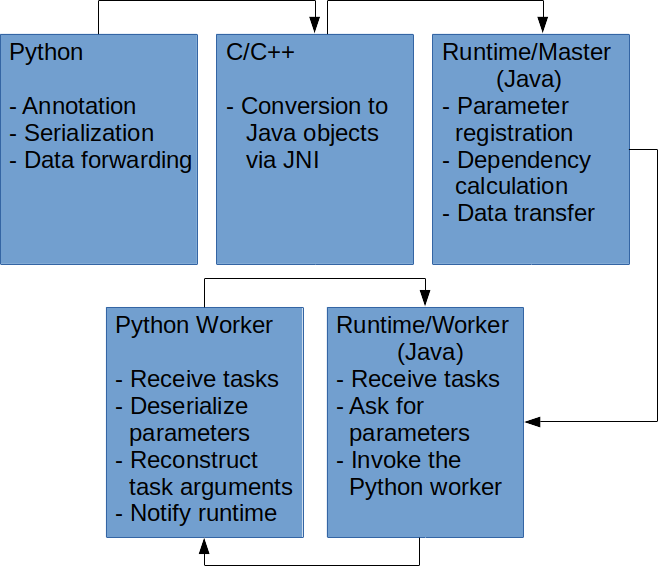
\includegraphics[scale = 0.5]{figures/parameter_pipeline.png}
\caption{The journey of a Python parameter, from the user's function call until the task in finished in the worker}
\label{fig:parameter_pipeline}
\end{figure}

In the following sections we will explain how the implementation of this feature affected all of the parts that appear in figure \ref{fig:parameter_pipeline}.

\subsubsection{Python Binding}
\label{subsubsec:python_binding_col_in}
This part covers intercepting the user's call to a PyCOMPSs task, the serialization of the task parameters (if necessary) and the forwarding of the necessary metadata to the Java Runtime.\\
\\
The very first step, and the easiest one, consists of adding a \verb|COLLECTION_IN| annotation in the list of annotations. This part is as easy as copy-pasting any of the existing parameters and then adapting it to our needs:

\inputminted{python}{snippets/param_col_in.py}

In fact, copy-pasting the specifications of the \verb|IN| parameter in more than enough. It is also necessary to add the type \verb|COLLECTION| in an inter-language type list which is after replicated in the three programming languages.\\
\\
The second step consists of serializing all the necessary data.

\inputminted{python}{snippets/serialize_object_into_file.py}

As we can see in the snippet, our implementation is just a recursive call to an already existing function devoted to serialize objects.

\subsubsection{C/C++ Bindings Common}
\label{subsubsec:bindings_common_col_in}
All metadata regarding parameters is produced by the corresponding binding (in our case, PyCOMPSs) and then translated to something understandable by the COMPSs runtime. This is achieved by extending Python with C++ and then sending messages via JNI (Java Native Interface \footnote{https://en.wikipedia.org/wiki/Java\_Native\_Interface}). In the case of the collection parameters it was decided to forward, from Python to Java, the following information:

\begin{verbatim}
collectionId N
type1 Val1
...
typeN ValN
\end{verbatim}

Note that if the $ith$ parameter is a collection then $val_i$ will contain the whole sub-collection.

\subsubsection{Runtime/Master (Java)}
\label{subsubsec:runtime_master_col_in}

%TODO: COLLECT DEPENDENCY GRAPH FROM MN3

\subsubsection{Runtime/Worker (Java)}
\label{subsubsec:runtime_worker_col_in}

\subsubsection{Python Worker}
\label{subsubsec:python_worker_col_in}
This last step is probably the easiest one. 


\subsection{Collections as INOUT Parameters}
\label{subsec:col_inout}

\subsection{Practical Applications}
\label{subsec:col_examples}
\subsection{Approximating cardinalities of huge sets}
\label{subsec:wcountproblem}
The Count-Distinct or Word Count Problem can be formulated as follows: given a sequence of elements $s_{1}, ..., s_{n}$ compute the amount of \textbf{distinct} elements in it. For example, for the sequence dog, cat, dog, bird, bird the answer is 3 (the distinct elements are bird, cat, and dog).

If the sequence is not too large this problem can be easily solved in expected linear time and space using hash tables, or $\mathcal{O}(nlogn)$ time and linear space using some data structures as Red-Black trees. However, this bound on space starts to become unacceptable when datasets are too large. In this section we will describe a probabilistic algorithm named as HyperLogLog \cite{Flajolet07hyperloglog:the}.\\
\\
This algorithm is very simple and yet very powerful. The core idea is the following: for each element $s_{i}$ of our sequence, use a hash function $h: \{0, 1\}^{*} \mapsto \{0, 1\}^b$ to compute a value $h(s_{i})$ and estimate the cardinality as $2^m$, where $m$ is the maximum number of leading zeros among all $h(s_{i})$. We must note that if all $h(x)$ have the same probability $\frac{1}{2^{b}}$ then the probability for some value to have $k$ leading zeros is $2^{-k}$. This means that the expected number of observations that are needed to find a number with $k$ leading zeros is $2^{k}$. Given that having a single hash value is not precise enough but computing multiple hash functions is too expensive, what is done is the following: 
\begin{enumerate}
\item Given a token $t$, compute $h(t)$
\item Take the first $p$ bits and use them to refer to a position in an array consisting of $2^p$ elements $a_{0}, ..., a_{2^p - 1}$
\item Update this position according to the other $b - p$ bits so it keeps the maximum amount of leading zeros seen so far
\item Once all tokens are processed output the harmonic mean of $2^{a_{0}}, ..., 2^{a_{2^p - 1}}$ as the answer.
\end{enumerate}
An interesting trivia fact is that if we need $\mathcal{O}(\log n)$ bits for our hash function to be able to count until $n$ then we only need $\mathcal{O}(\log \log n)$ to store the number of leading zeros of some hash value. This is why HyperLogLog is called that way.\\
\\
A very nice property of HyperLogLog is that two distinct runs on two different datasets can be merged if they have used the same parameters (hash function, $b$, and $p$) in such a way that it approximates the cardinality of the union of the two datasets. Given two arrays $a$ and $b$, each corresponding to a run of HyperLogLog we can get a fictional run of HyperLogLog $c$ that represents the union of both datasets by computing $c_{i} =\max(a_{i}, b_{i})$ for all of the $2^{p}$ positions. This makes sense, as it produces the same result as running a single HyperLogLog on the concatenation of the two datasets. This property allows us to parallelize or to distribute this algorithm, giving us a potential performance boost. The source code we will use for our experiments can be found in appendix \ref{subsec:hyperloglog_source_code}.\\
\\
Note that this application is a classical \textit{map-reduce} workflow. Without collections we are forced to implement any reduce function as \verb|reduce(f, *args)|. Each extra argument is passed as an input parameter via socket and pipe, implying a huge overhead. With collections only the collection object, and the list of identifiers, are transferred. The other properties of the contents, such as direction, locations and so on, are deduced or requested in the destination node.\\
\\
The elimination of this overhead is noticeable even with a very small number of parameters. As we can see in figure \ref{fig:collection_vs_normal}, the collection feature reduces the overhead drastically. An important observation is that a PyCOMPSs task of the form \verb|f(*args)| usually starts to show problems and crashes when more than $60$ arguments are passed, as each argument represents a lot of metadata to be transferred via socket and pipe.
\begin{figure}[ht!]
\centering
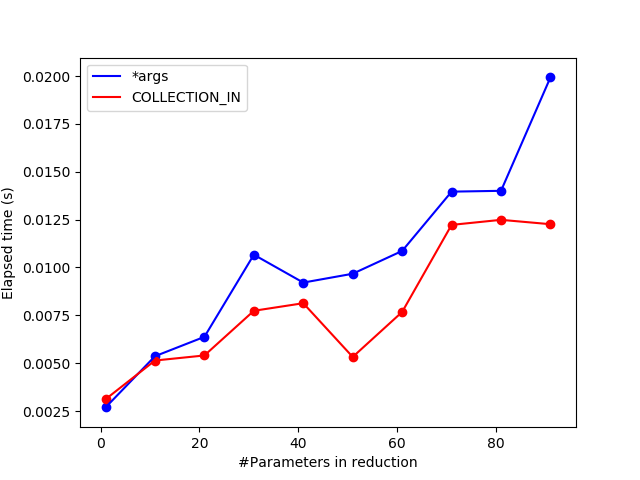
\includegraphics[scale = 0.5]{figures/collection_vs_normal.png}
\caption{Execution time of the reduce functions with and without collections. Each point is the average of 5 executions. Although the samples are noisy, as they are small, a consistent improvement by the collection feature can be appreciated. The non-collections versions started to crash and to show strange behaviours around the 60 parameters}
\label{fig:collection_vs_normal}
\end{figure}\\
\\
A comparison between the amount of meta-data generated and sent by the classical reduce implementation and by the collections version can be found in appendix \ref{subsec:reduce_data_comparison}.

This improvement benefits many applications, as the map-reduce scheme is very common.